% Sketch output, version 0.3 (build 7d, Wed Dec 12 14:04:11 2012)
% Output language: PGF/TikZ,LaTeX
\documentclass[letterpaper,12pt]{article}
\usepackage[x11names,rgb]{xcolor}
\usepackage{tikz}
\usetikzlibrary{snakes}
\usetikzlibrary{arrows}
\usetikzlibrary{shapes}
\usetikzlibrary{backgrounds}
\usepackage{amsmath}
\oddsidemargin 0in
\evensidemargin 0in
\topmargin 0in
\headheight 0in
\headsep 0in
\textheight 9in
\textwidth 6.5in
\begin{document}
\pagestyle{empty}
\vspace*{\fill}
\begin{center}
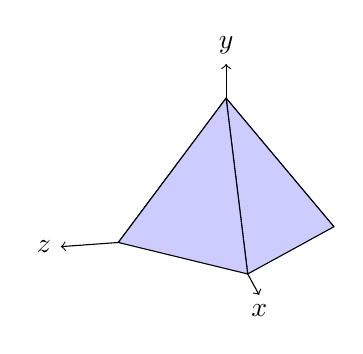
\begin{tikzpicture}[line join=round]
\filldraw[fill=blue!20](0,1.733)--(-1.369,-.1)--(-.274,.5)--(0,1.733)--cycle;
\filldraw[fill=blue!20](0,1.733)--(-.274,.5)--(1.369,.1)--(0,1.733)--cycle;
\filldraw[fill=blue!20](0,1.733)--(1.369,.1)--(.274,-.5)--(0,1.733)--cycle;
\draw[arrows=-,line width=.4pt](.274,-.5)--(0,0)--(0,1.733);
\draw[arrows=-,line width=.4pt](0,0)--(-1.369,-.1);
\filldraw[fill=blue!20](0,1.733)--(.274,-.5)--(-1.369,-.1)--(0,1.733)--cycle;
\draw[arrows=->,line width=.4pt](-1.369,-.1)--(-2.1,-.153);
\draw[arrows=->,line width=.4pt](0,1.733)--(0,2.167);
\draw[arrows=<-,line width=.4pt](.42,-.767)--(.274,-.5);
\path (-2.1,-.153) node[left] {$z$}
                   (.42,-.767) node[below] {$x$}
                   (0,2.167) node[above] {$y$};\end{tikzpicture}
\end{center}
\vspace*{\fill}
\end{document}
% End sketch output
